% ALGUNOS PAQUETES REQUERIDOS (EN UBUNTU): %
% ========================================
% %
% texlive-latex-base %
% texlive-latex-recommended %
% texlive-fonts-recommended %
% texlive-latex-extra %
% texlive-science %
% texlive-lang-spanish (en ubuntu 13.10) %
% ******************************************************** %

\documentclass[a4paper]{article}
\usepackage[spanish, es-nodecimaldot]{babel}
\usepackage[utf8]{inputenc}
\usepackage{fancyhdr}
\usepackage[pdftex]{graphicx}
\usepackage{sidecap}
\usepackage{caption}
\usepackage{subcaption}
\usepackage{booktabs}
\usepackage{makeidx}
\usepackage{float}
\usepackage{amsmath, amsthm, amssymb}
\usepackage{amsfonts}
\usepackage{sectsty}
\usepackage{wrapfig}
\usepackage{listings}
\usepackage{pgfplots}
\usepackage{pgfplotstable}
\usepackage{enumitem}
\usepackage[hidelinks]{hyperref}
\usepackage{listings}
\usepackage{listingsutf8}

\linespread{factor}

\definecolor{mygreen}{rgb}{0,0.6,0}
\definecolor{mygray}{rgb}{0.5,0.5,0.5}
\pgfplotsset{compat=1.8}
\setlist[enumerate]{label*=\arabic*.}
\lstset{
	inputencoding=utf8/latin1,
	language=C++,
	basicstyle=\ttfamily,
	keywordstyle=\bfseries\color{blue},
	stringstyle=\color{red}\ttfamily,
	commentstyle=\color{mygreen}\ttfamily,
	morecomment=[l][\color{magenta}]{\#},
	numbers=left,
	numberstyle=\color{mygray}
}

\usepackage{fancyhdr}
\pagestyle{fancy}
\fancyhf{}
\fancyhead[LO]{Problemas, Algoritmos y Programación}
\fancyhead[RO]{Trabajo Práctico N\textsuperscript{o} 1}
\fancyfoot[LO]{\small{Shai Bianchi, Martín Jedwabny, Manuel Mena, Iván Pondal}}
\fancyfoot[RO]{\thepage}
\renewcommand{\headrulewidth}{0.5pt}
\renewcommand{\footrulewidth}{0.5pt}
\setlength{\textwidth}{16cm}
\setlength{\hoffset}{-1.1cm}
\setlength{\headsep}{0.5cm}
\setlength{\textheight}{25cm}
\setlength{\voffset}{-1.75cm}
\setlength{\headwidth}{\textwidth}
\setlength{\headheight}{13.1pt}
\renewcommand{\baselinestretch}{1.1} % line spacing

\usepackage{caratula}

\allowdisplaybreaks
\newcommand{\ord}{\ensuremath{\operatorname{O}}}
\newcommand{\nat}{\ensuremath{\mathbb{N}}}
\newcommand{\acr}[1]{\lowercase{\textsc{#1}}}
\newcommand{\comp}{\ensuremath{^{\operatorname{C}}}}
\newcommand{\argmax}{\operatornamewithlimits{arg\,m\acute{a}x}}

\newcommand{\subheading}[1]{\vspace{1em} \noindent\textbf{#1} \nopagebreak
\smallskip \nopagebreak}

% Lemas, definiciones, etc.
\theoremstyle{plain}
  \newtheorem{prop}{Proposición}
  \newtheorem{lema}{Lema}
\theoremstyle{remark}
  \newtheorem{obs}{Observación}
\theoremstyle{definition}
  \newtheorem{defi}{Definición}

% Pseudocódigo
\usepackage[onelanguage, spanish]{algorithm2e}
    % \NoCaptionOfAlgo
    \LinesNumbered\RestyleAlgo{ruled}\IncMargin{1em}\DontPrintSemicolon
    \SetArgSty{}\SetCommentSty{textsf}\SetFuncSty{textsf}
    \SetKwInput{Input}{Entrada}
    \SetKwInput{Output}{Salida}
    \SetKwProg{For}{para}{ hacer}{fin}
    \SetKwProg{Fn}{función}{:}{fin}

\begin{document}
\materia{Problemas, Algoritmos y Programación}
\submateria{Segundo cuatrimestre de 2016}
\titulo{Trabajo Práctico N\textsuperscript{o} 1}
\integrante{Shai Bianchi}{540/12}{bianchishai@gmail.com}
\integrante{Martín Jedwabny}{885/13}{martiniedva@gmail.com}
\integrante{Manuel Mena}{313/14}{manuelmena1993@gmail.com}
\integrante{Iván Pondal}{078/14}{ivan.pondal@gmail.com}

%\maketitle
% no footer on the first page

% group hash
% seed = 2^32 + 42
\vspace*{\fill}
\begin{center}
8796613900571664
\end{center}
\vspace*{\fill}

\thispagestyle{empty}

\newpage
\tableofcontents

\newpage
\section{Ejercicio 2}

\subsection{Problema}
El enunciado explica un problema en el cual tengo una cierta cantidad de
`amigas' de Lisa $N$ y para cada una de ellas sabemos la diversión que cada par
de amigas aporta a una fiesta. Luego nos pide hallar la máxima diversión que se
puede obtener separando a sus amigas en `fiestas' donde cada fiesta le aporta la
diversión que suman las amigas que están en ella. \\ Yendo al algoritmo, tenemos
como entrada un valor entero positivo $N$ y una
matriz $D$ de $N \times N$ simétrica con valores enteros y diagonal 0.

Esto tiene sentido ya que una amiga no aporta diversión consigo misma (por eso
la diagonal en 0) y la diversión que aporta una amiga $j$ con otra amiga $t$ es
la misma diversión que aporta $t$ con $j$ (por eso es simétrica).

Tal como relata el problema, $N$ es la cantidad de amigas de Lisa y la matriz
$D$ nos dice para cada $t,j \in [1..n]$ la diversión que aportan las amigas $t$
y $j$ si se encontraran en la misma fiesta.

Dado el conjunto $A = \{1,...,N\}$ (que usaremos para representar a las amigas
de Lisa) y una partición $B = \{A_1,...,A_k\}$ de A, definimos $B_D$ la `suma de
una partición sobre $D$' como:

\begin{equation*}
    B_D = \sum_{i=1}^{k}{\sum_{j \in A_i}^{}{\sum_{t \in A_i : t < j}^{}{D_{t,j}}}}
\end{equation*}

Es decir, $B_D$ es la suma de $D_{t,j}$ para todo $t$ y $j$ que pertenecen al
mismo subconjunto en la partición $B$, la condición $t < j$ me asegura no
considerar $D_{t,j}$ y $D_{j,t}$ ya que la matriz es simétrica y solo me
interesa considerar cuánto le aporta a la `suma' el par una sola vez.

A su vez, $B_D$ representa cuánta diversión tendríamos si separáramos a las
amigas de Lisa en fiestas diferentes mediante la partición $B$.

Habiendo definido eso, quiero hallar el máximo $B_D$ para cualquier partición
$B$ de $A$, mejor dicho, la máxima `suma de una partición sobre D' de $A$
posible, lo cual representaría la forma de separar a las amigas de Lisa en
fiestas para que la suma de la diversión que aportan sea máxima.

\subsection{Algoritmo e intuición}

\subsubsection*{Pseudocódigo}

\begin{algorithm}[H]
    \caption{MáximaSumaPartición}
    \Input{Entero positivo $N$ y Matriz $D$ simétrica de enteros con diagonal 0}
    $int$  $\mathit{dp[1<<N]} \gets [-1,...,-1]$ \;
    $\mathit{dp[0]} \gets 0$ \;
    \Return{\emph{MáximaSumaParticiónParaSubconjunto}$(N,D,dp,(1<<N)-1)$}
\end{algorithm}

\begin{algorithm}[H]
    \caption{MáximaSumaParticiónParaSubconjunto}
    \Input{Entero positivo $N$, Matriz $D$ simétrica de enteros con diagonal 0, Arreglo $dp$ de tamaño $2^N$ y Mascara de bits $mask$}
    \eIf{$\mathit{dp[mask]}$ != $-1$} {
        \Return{$\mathit{dp[mask]}$}
    }{
    int $\mathit{res} \gets 0$ \;
    \For {int $i \gets 0$ ; $i < N$; $i \gets i + 1$} {
        \For {int $j \gets 0$ ; $j < i$; $j \gets j + 1$} {
            \If {($mask$ \& (($1 << i$) $\|$ ($1 << j$))) $==$ (($1 << i$) $\|$ ($1 << j$))} {
                $res$ $+=$ $D_{i,j}$
            }
        }
    }
    $res \gets max(res, 0)$ \;
    \For {int $s1 \gets mask \& (mask-1)$; $s1$ != $0$; $s1 \gets mask \& (s1-1)$} {
        int $s2 \gets mask \& ($ $NOT$ $ s1)$ \;
        int $c1$ = \emph{MáximaSumaParticiónParaSubconjunto}$(N, D, dp, s1)$ \;
        int $c2$ = \emph{MáximaSumaParticiónParaSubconjunto}$(N, D, dp, s2)$ \;
        $res \gets max(res, c1+c2)$ \;
    }
    $dp[mask] \gets res$ \;
    \Return{$res$}
    }
\end{algorithm}
\bigskip

\subsubsection*{Estrategia}

Nuestro algoritmo usa la estrategia de Programación Dinámica para iterar
conjuntos que representamos con máscaras de bits. Comenzamos llamando a la
función recursiva \emph{MáximaSumaParticiónParaSubconjunto} con la máscara que
representa al conjunto entero y le pedimos la máxima diversión que pueden
aportar.

Luego la función recursiva se fija para todos sus particiones
posibles, de qué forma puede dividir el conjunto tal que la diversión que
aporten los subconjuntos de la partición sea máxima. Nuevamente, esto lo hacemos
representando los subconjuntos con máscaras de bits y recorriendo los
subconjuntos de cada conjunto de la forma que explicaron en clase.

\subsection{Correctitud}

\subsubsection*{MáximaSumaPartición}
Tal como vimos en ejemplos en clase, inicializamos un arreglo de soluciones para
todos los subconjuntos posibles de `amigas de Lisa' que llamamos $dp$, donde
$dp[mask]$ al final del algoritmo nos debería haber calculado para el
subconjunto de amigas que representa `mask', la máxima suma posible de diversión
que pueden aportar esas amigas repartiéndolas (particionándolas) en fiestas.

Inicialmente queremos calcular la máxima diversión que puede obtenerse mediante
todas las amigas de Lisa, lo cual representamos mediante la máscara de bits
`11...1' (donde la cantidad de 1s es N), lo cual escribimos como $(1<<N)-1$.

Dada esta preparación le mandamos $dp$ y la máscara inicial al algoritmo
\emph{MáximaSumaParticiónParaSubconjunto} que calcula la máxima diversión para todas
las amigas de Lisa.

\subsubsection*{MáximaSumaParticiónParaSubconjunto}

En este algoritmo, dadas las soluciones recursivas ya calculadas en el arreglo
de enteros $dp$, toma una máscara de bits $mask$ y calcula la máxima diversión
que pueden aportar las amigas de Lisa que representa $mask$.

En primer lugar nos fijamos si la solución ya fue calculada previamente en $dp$
y si lo fue la devolvemos. En caso contrario, calculamos tres cosas:

\begin{itemize}
    \item [$res \gets 0$] El caso en que todas las amigas van a fiestas distintas (la diversión sería 0).
    \item [For 1] Cuando todas las amigas de el subconjunto actual van a la misma fiesta (lo que calculamos con el primer ciclo For). Acá lo que tenemos que hacer es simplemente recorrer cada par $i,j$ con $i,j \in [1..N]$ (pero no el par $j,i$, lo cual ya explicamos al comienzo) y sumar la diversión que aportan si es que las amigas $i$ y $j$ de Lisa están en el subconjunto actual. Ver que están en el subconjunto actual (representado por $mask$) lo podemos ver exactamente de la misma forma que lo hicimos en clase: \\
    ($mask$ \& (($1 << i$) $\|$ ($1 << j$))) $==$ (($1 << i$) $\|$ ($1 << j$)).
    \item [For 2] Vemos para cada subconjunto propio del conjunto actual cuánta diversión puedo obtener si separo el conjunto actual en dos: el subconjunto propio y su complemento (que obtenemos con $s2 \gets mask \& ($ $NOT$ $ s1)$). Con esto hacemos dos llamados recursivos a esta misma función y comparamos qué forma de partir el conjunto actual nos puede terminar aportando más diversión. Es importante ver que de esta manera recorremos todas las particiones posibles del conjunto actual ya que si bien en este ciclo For separamos el conjunto en dos de todas las formas posibles, cuando hago las llamadas recursivas, estos subconjuntos serán también particionados de todas las formas posibles. Como vimos en clase, recorrer los subconjuntos de un conjunto se puede hacer con: \\
    int $s1 \gets mask$; $s1$ != $0$; $s1 \gets mask \& (s1-1)$ \\
    Pero en este código queremos recorrer los subconjuntos propios, por lo cual lo modificamos a: \\
    int $s1 \gets mask \& (mask-1)$; $s1$ != $0$; $s1 \gets mask \& (s1-1)$ \\
    Que simplemente comienza con el primer subconjunto diferente al conjunto actual.
\end{itemize}

De esas tres opciones elegimos como solución la que más diversión aporta.

Finalmente guardamos la solución para el subconjunto actual en el arreglo $dp$ y la devolvemos como respuesta.

\subsection{Complejidad}

Recorremos todas las $2^N$ instancias representadas con las máscaras de bits
mediante llamados recursivos, pero no más que eso porque guardamos las
respuestas ya calculadas con Programación Dinámica mediante un arreglo.

Por cada instancia tenemos algunas asignaciones y dos ciclos For.

El primer ciclo itera $O(n^2)$ combinaciones de indices y adentro realiza
comparaciones y asignaciones por lo cual su complejidad es de $O(n^2)$.

El segundo ciclo itera cada subconjunto del conjunto actual y adentro realiza
(además de los llamados recursivos, que eso lo consideramos aparte al principio
cuando dijimos que iteramos los $2^N$ subconjuntos posibles), solamente
asignaciones y otras operaciones básicas.

Como vimos en clase, si para cada instancia de las $2^N$ que existen iteramos
sus subconjuntos, nos da una complejidad de $O(3^N)$.\\ Además, por cada una de
las instancias realizamos $O(n^2)$ operaciones mediante el primer For, lo cual
conlleva una complejidad de $O(2^n * n^2) = O(3^n)$.

En total tendríamos una complejidad de $O(3^n) + O(3^n) = O(3^n)$, tal como pide
el enunciado.

\subsection{Casos de prueba}

En primera instancia comprobamos que el algoritmo devuelva la salida correcta para los casos provistos por la cátedra. \\
Luego generamos nuestras propias instancias bajo las condiciones del enunciado, es decir, matrices cuadradas y simétricas con diagonal 0 de tamaño menor o igual a 18. \\
Mediante estos, comprobamos no solo la correctitud misma del algoritmo sino también casos borde 
(por ejemplo, que todas las amigas de Lisa se lleven mal entre sí) 
y que no tarde demasiado en encontrar una respuesta para instancias grandes.


\subsubsection*{Caso 1}

\textbf{Motivo}: Comprobamos que el algoritmo funcione correctamente en una instancia un poco mas grande que las provistas por la cátedra. \\

\textbf{Entrada}:

\begin{flushleft}
$\qquad N = 5$\\[10pt]
$\qquad D = \left( \begin{smallmatrix}
0 & 2 & 2 & -1 & 2 \\
2 & 0 & -10 & 1 & 1 \\
2 & -10 & 0 & -2 & 2 \\
-1 & 1 & -2 & 0 & 3 \\
2 & 1 & 2 & 3 & 0 \\
\end{smallmatrix} \right)$
\end{flushleft}

\textbf{Resultado}: El algoritmo nos dio como resultado 8 y lo hizo de manera inmediata. Esto tiene sentido ya 
que es una instancia chica y llegamos a esa solución tomando las amigas $\{ 0, 1, 3, 4 \}$ en una fiesta y $\{ 2 \}$ en otra fiesta.

\subsubsection*{Caso 2}

\textbf{Motivo}: Comprobamos el funcionamiento del algoritmo para una instancia un poco más grande donde tenemos 3 clanes de amigas de Lisa bien definidos. 
Cada clan es de 4 amigas que se llevan bien entre sí pero con nadie más de otros clanes. \\

\textbf{Entrada}:

\begin{flushleft}
$\qquad N = 12$\\[10pt]
$\qquad D = \left( \begin{smallmatrix}
0 & 1 & 1 & 1 & -1 & -1 & -1 & -1 & -1 & -1 & -1 & -1 \\
1 & 0 & 1 & 1 & -1 & -1 & -1 & -1 & -1 & -1 & -1 & -1 \\
1 & 1 & 0 & 1 & -1 & -1 & -1 & -1 & -1 & -1 & -1 & -1 \\
1 & 1 & 1 & 0 & -1 & -1 & -1 & -1 & -1 & -1 & -1 & -1 \\
-1 & -1 & -1 & -1 & 0 & 1 & 1 & 1 & -1 & -1 & -1 & -1 \\
-1 & -1 & -1 & -1 & 1 & 0 & 1 & 1 & -1 & -1 & -1 & -1 \\
-1 & -1 & -1 & -1 & 1 & 1 & 0 & 1 & -1 & -1 & -1 & -1 \\
-1 & -1 & -1 & -1 & 1 & 1 & 1 & 0 & -1 & -1 & -1 & -1 \\
-1 & -1 & -1 & -1 & -1 & -1 & -1 & -1 & 0 & 1 & 1 & 1 \\
-1 & -1 & -1 & -1 & -1 & -1 & -1 & -1 & 1 & 0 & 1 & 1 \\
-1 & -1 & -1 & -1 & -1 & -1 & -1 & -1 & 1 & 1 & 0 & 1 \\
-1 & -1 & -1 & -1 & -1 & -1 & -1 & -1 & 1 & 1 & 1 & 0 \\
\end{smallmatrix} \right)$
\end{flushleft}

\textbf{Resultado}: El algoritmo nos dio como resultado 18 y lo hizo de manera casi inmediata (no lento, pero no
 tan instantáneo como el caso anterior). Como podíamos predecir, el algoritmo nos da el resultado de agrupar 
 cada uno de los 3 clanes de los que hablábamos previamente. Cada amiga en un clan aporta 1 punto de diversión 
 con las demás, por lo tanto un clan de 4 amigas suma en total 6 puntos de diversión, es decir el número 
 combinatorio (4,2) que son las formas de tomar 2 amigas de un clan de 4. Si sumamos la diversión de cada fiesta
 de cada clan nos da $3 * 6 = 18$ unidades de diversión.

\subsubsection*{Caso 3}

\textbf{Motivo}: Queremos comprobar cuánto tiempo tarda el algoritmo para una instancia de tamaño máximo y ver el resultado para el caso en que ninguna amiga de Lisa se lleva bien con las demás.

\textbf{Entrada}:

\begin{flushleft}
$\qquad N = 18$\\[10pt]
$\qquad D = \left( \begin{smallmatrix}
0 & -1 & -1 & -1 & -1 & -1 & -1 & -1 & -1 & -1 & -1 & -1 & -1 & -1 & -1 & -1 & -1 & -1 \\
-1 & 0 & -1 & -1 & -1 & -1 & -1 & -1 & -1 & -1 & -1 & -1 & -1 & -1 & -1 & -1 & -1 & -1 \\
-1 & -1 & 0 & -1 & -1 & -1 & -1 & -1 & -1 & -1 & -1 & -1 & -1 & -1 & -1 & -1 & -1 & -1 \\
-1 & -1 & -1 & 0 & -1 & -1 & -1 & -1 & -1 & -1 & -1 & -1 & -1 & -1 & -1 & -1 & -1 & -1 \\
-1 & -1 & -1 & -1 & 0 & -1 & -1 & -1 & -1 & -1 & -1 & -1 & -1 & -1 & -1 & -1 & -1 & -1 \\
-1 & -1 & -1 & -1 & -1 & 0 & -1 & -1 & -1 & -1 & -1 & -1 & -1 & -1 & -1 & -1 & -1 & -1 \\
-1 & -1 & -1 & -1 & -1 & -1 & 0 & -1 & -1 & -1 & -1 & -1 & -1 & -1 & -1 & -1 & -1 & -1 \\
-1 & -1 & -1 & -1 & -1 & -1 & -1 & 0 & -1 & -1 & -1 & -1 & -1 & -1 & -1 & -1 & -1 & -1 \\
-1 & -1 & -1 & -1 & -1 & -1 & -1 & -1 & 0 & -1 & -1 & -1 & -1 & -1 & -1 & -1 & -1 & -1 \\
-1 & -1 & -1 & -1 & -1 & -1 & -1 & -1 & -1 & 0 & -1 & -1 & -1 & -1 & -1 & -1 & -1 & -1 \\
-1 & -1 & -1 & -1 & -1 & -1 & -1 & -1 & -1 & -1 & 0 & -1 & -1 & -1 & -1 & -1 & -1 & -1 \\
-1 & -1 & -1 & -1 & -1 & -1 & -1 & -1 & -1 & -1 & -1 & 0 & -1 & -1 & -1 & -1 & -1 & -1 \\
-1 & -1 & -1 & -1 & -1 & -1 & -1 & -1 & -1 & -1 & -1 & -1 & 0 & -1 & -1 & -1 & -1 & -1 \\
-1 & -1 & -1 & -1 & -1 & -1 & -1 & -1 & -1 & -1 & -1 & -1 & -1 & 0 & -1 & -1 & -1 & -1 \\
-1 & -1 & -1 & -1 & -1 & -1 & -1 & -1 & -1 & -1 & -1 & -1 & -1 & -1 & 0 & -1 & -1 & -1 \\
-1 & -1 & -1 & -1 & -1 & -1 & -1 & -1 & -1 & -1 & -1 & -1 & -1 & -1 & -1 & 0 & -1 & -1 \\
-1 & -1 & -1 & -1 & -1 & -1 & -1 & -1 & -1 & -1 & -1 & -1 & -1 & -1 & -1 & -1 & 0 & -1 \\
-1 & -1 & -1 & -1 & -1 & -1 & -1 & -1 & -1 & -1 & -1 & -1 & -1 & -1 & -1 & -1 & -1 & 0 \\
\end{smallmatrix} \right)$
\end{flushleft}

\textbf{Resultado}: El algoritmo nos dió como resultado 0, lo cual era de esperarse ya que ninguna amiga de Lisa 
se llevaba bien con las demás y por lo tanto se deben separar en una fiesta por amiga. En cuanto al tiempo que 
tardó en dar esta respuesta fue de un par de segundos, lo cual indica que el tiempo aumenta bastante a medida 
que crecen las instancias pero aún asi lo resuelve en tiempo razonable para las cotas dadas por la cátedra.


\newpage
\subsection{Problema}
Dado un arreglo de números enteros de entrada, se pide encontrar la máxima suma posible de elementos correspondientes a subarreglos contiguos de dicha entrada. Se considera que el arreglo vacío tiene suma nula y que cumple ser un subarreglo contiguo de todo arreglo. Consideraremos que un \textit{subarreglo} siempre es contiguo. Además, nos referirimos a la suma de los elementos de un subarreglo como \textit{la suma del subarreglo}.

\subsection{Algoritmo e intuición}

\noindent Entrada: \textit{A} \newline
\textit{acumulador}, \textit{máximo} $\leftarrow 0$ \newline
\textbf{para} x \textbf{en} \textit{A} \textbf{hacer} \newline
\indent $\mathit{acumulador} \leftarrow \mathit{acumulador + x}$ si es positivo, $0$ de lo contrario \newline
\indent \textit{máximo} $\leftarrow$ el máximo entre \textit{máximo} y $\mathit{acumulador}$

\bigskip

Nuestro algoritmo itera los elementos del arreglo recorriéndolo de principio a fin una sola vez. En cada iteración, suma en un acumulador inicializado en cero el elemento correspondiente, siempre que al sumarlo la acumulación resulte positiva; de lo contrario, vuelve a poner el acumulador en cero. De esta forma, en la iteración $k$, \textit{acumulador} tiene el valor de la suma o bien de un subarreglo cuyo último elemento es el $k-1$\textit{-ésimo} del arreglo, o bien la del subarreglo vacío. Además, el algoritmo tiene en \textit{máximo} luego de cada iteración un registro del máximo valor de acumulación conseguido hasta ese momento.

La intuición detrás del algoritmo es que, mientras un subarreglo en particular sume una cantidad positiva, tiene sentido seguir considerándolo como el prefijo de un subarreglo candidato a realizar la suma óptima, ya que esa cantidad positiva puede aportar una cantidad útil a lo que sumen los elementos que siguen; en cambio, al ser negativa la suma de un subarreglo, no tiene sentido verlo como prefijo de un subarreglo candidato ya que su suma sólo le restaría a lo que puedan aportar los elementos que le siguen. En este sentido, el poner en cero el acumulador luego de encontrar una acumulación negativa equivale a descartar los subarreglos que se estaban evaluando desde la última vez que el acumulador se puso en cero y empezar a evaluar subarreglos que comienzan inmediatamente después del descartado.

Para verlo en más detalle, supongamos el caso de un arreglo $A$ para el cual el algoritmo vuelve a poner en cero su acumulador por primera vez en la iteración $i_1 > 0$. Es decir, el prefijo de longitud $i_1$ de $A$ es el primer subarreglo de suma negativa que nuestro algoritmo contempla. Notar que esto requiere que el último elemento de dicho prefijo sea un número negativo de módulo mayor a la suma del prefijo de $A$ de longitud $i_1-1$. Si luego el algoritmo vuelve encontrar una acumulación negativa en la iteración $i_2 > i_1$, tenemos que vuelve a poner en cero su acumulador luego del prefijo de $A$ de longitud $i_1 + i_2$, formado por el prefijo de $A$ de longitud $i_1$ y los $i_2$ elementos que le siguen, cuya suma también es negativa. Nuevamente, el elemento $i_2$\textit{-ésimo} deberá ser un entero negativo de módulo mayor al de la suma de los $i_2-i_1-1$ que lo preceden. Si luego ocurre lo análogo para un índice $i_3 > i_2$, tendremos que el algoritmo vuelve a anular su acumulador luego del prefijo de longitud $i_1 + i_2 + i_3$ de $A$ que suma una cantidad negativa también y cuyo último elemento es un negativo de módulo mayor a la suma de sus $i_3-i_2-1$ anteriores, y así.

\subsection{Correctitud}

Sea $A$ un arreglo y $s$ el resultado correcto del problema para $A$, es decir, la máxima suma posible para subarreglos de $A$. Esta cantidad óptima existe ya que el conjunto de posibles sumas de subarreglos es un conjunto finito de números enteros y por ende tiene un máximo. Observemos que $s$ nunca será un valor negativo ya que todo arreglo tiene un subarreglo vacío cuya suma es nula, en cuyo caso se tendría una suma de un subarreglo mayor a $s$ lo cual sería absurdo habiend supuesto óptimo a $s$.

Sea además $S$ un subarreglo minimal de $A$ que realiza la suma óptima $s$ y tal que su primer elemento está en la posición $i$ de $A$. Notar que ningún prefijo de $S$ puede tener una suma negativa, ya que de tenerla, podríamos tomar el sufijo maximal de $S$ que tenga una suma mayor o igual a $0$ y conseguiríamos con ese subarreglo una suma mayor a $s$, siendo que $s$ contendrá en su suma el mencionado prefijo negativo y el sufijo maximal no, lo cual daría un absurdo dado que $s$ se supuso óptimo.

Vamos a ver la correctitud de nuestro algoritmo demostrando que el mismo necesariamente considera la suma del subarreglo $S$ como candidata. Primero, demostramos que el algoritmo comienza a iterar los elementos de $S$ teniendo \textit{acumulador} en $0$.

\begin{itemize}
    \item \textbf{Caso} $\mathbf{i = 0}$. En este caso, el subarreglo $S$ es un prefijo de $A$. Por lo tanto, nuestro algoritmo lo contempla necesariamente ya que comienza a iterar al principio de $A$, y lo hace con \textit{acumulador} en $0$ dado que se inicializa en ese valor.

    \item \textbf{Caso} $\mathbf{i > 0}$. Sea $S_{pre}$ el prefijo de $A$ cuyo último elemento es el $i-1$\textit{-ésimo} de $A$. En este caso, todo sufijo de $S_{pre}$ suma necesariamente una cantidad menor o igual a $0$, ya que si existiera uno que suma una cantidad positiva, podríamos tomar el subarreglo que resulta de concatenar ese sufijo con $S$ y obtener una suma mayor a $s$. Por lo tanto, podemos afirmar que al comenzar a recorrer el subarreglo $S$, \textit{acumulador} está en $0$.
\end{itemize}

Como $S$ no tiene prefijos que sumen una cantidad negativa o nula, una vez que el ciclo comienza a iterar sus elementos \textit{acumulador} nunca se pondrá en cero hasta terminar de recorrer $S$. Por ende, en ese punto, \textit{máximo} tendrá el valor $s$. Además, dicha variable sólo cambia de valor en iteraciones en las que \textit{acumulador} tiene un valor mayor aún. Dado que \textit{acumulador} sólo toma valores de sumas de subarreglos de $A$ y siendo por hipótesis $s$ mayor o igual a todos esos valores, podremos concluir que, al finalizar la ejecución del ciclo, \textit{máximo} es igual a $s$. Como el valor de retorno del algoritmo es el que tiene \textit{máximo} luego del ciclo, el mismo devuelve $s$.

\subsection{Casos de prueba}


\newpage
\section{Ejercicio 4}

\subsection{Introducción}

Para este ejercicio se pedía dado un arreglo de $N$ matrices en
$\mathbb{Z}_{10007}^{3 \times 3}$ decidir si existía un subarreglo de longitud
$L$ tal que su producto fuera igual a $M \in \mathbb{Z}_{10007}^{3 \times 3}$.
Además, el algoritmo desarrollado debía tener una complejidad temporal $\ord(N
\times \log N)$.

\subsection{Solución propuesta}\label{ej4:sol}

La solución desarrollada hace uso de la técnica de \emph{Divide \& Conquer}.
Esto se debe a que el problema tiene la característica de poder ser dividido en
subproblemas más pequeños que unidos resuelven lo pedido.

Si existe el subarreglo cuyo producto corresponde a $M$ es bajo alguna de
las siguientes posibilidades:

\begin{itemize}
	\item El subarreglo existe en $\left[ 0,\frac{N}{2} \right)$.
	\item El subarreglo existe en $\left[\frac{N}{2}, N \right)$.
	\item El subarreglo está atravesando ambas mitades.
\end{itemize}

En caso de no cumplirse ninguna de estas opciones el subarreglo pedido no
existe.

De esta forma se puede ver entonces cómo partiendo el arreglo en dos
mitades el ejercicio se puede resolver llamando el algoritmo de forma recursiva
sobre cada una y estudiando el caso donde atraviesa a ambas.

El escenario que requiere mayor atención es el del subarreglo atravesando ambas mitades.
Para ello, es necesario probar el producto de todo subarreglo de longitud $L$
que se encuentre atravesando ambas mitades.

Una implementación básica simplemente intentaría multiplicar desde la posición
más a la izquierda tal que el subarreglo resultante de tamaño $L$ atravesara la
mitad. Luego, si el producto fuera distinto a $M$, se iría corriendo de a un
lugar a la derecha repitiendo el proceso hasta que ya no fuera posible o
encontrase el subarreglo buscado. Esta operación sería cuadrática en el tamaño
de $L$, que al estar acotado por $N$ resulta en una complejidad temporal
$\ord(N^{2})$. Como esta cota supera la requerida por el ejercicio fue necesario
optimizar esta operación.

Dado que el producto de matrices es asociativo, teniendo un subarreglo de tamaño
$L$ con elementos $M_k \dots M_{k + L - 1}$ su producto se puede calcular
mediante:

\begin{gather*}
	\left(M_k \times M_{k + 1} \times \dots \times M_m\right) \times
		\left(M_{m + 1} \times M_{m + 2} \times \dots \times M_{k + L - 1}\right) \\
		\left(\forall m\right) k \leq m \leq k + L - 1
\end{gather*}

Entonces, si definimos $m = \frac{N}{2}$ el producto de todos los subarreglos de
tamaño $L$ que atraviesan ambas mitades se puede calcular como el de las
matrices de la mitad izquierda por el de las de la derecha.

Para reducir el número de operaciones lo que se hace es para cada mitad ya tener
calculados los productos de matrices desde la mitad hacia el extremo del
arreglo. Cuando se realiza la llamada recursiva a la función, además de pasar el
intervalo del arreglo sobre el cual operar, se indica mediante una bandera si se
trata de la mitad derecha o la izquierda. Si se trata de la mitad derecha los
productos se calculan desde el primer elemento hacia el último, caso
contrario, del último a el primero.

Esta operación tiene un costo $\ord(N)$ ya que para cada posición del arreglo se
calcula y almacena el producto entre la matriz en ese punto y el producto hasta
la posición anterior.

\begin{figure}[H]
	\centering
	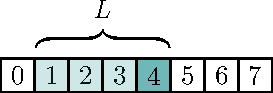
\includegraphics{imagenes/subarray_product_across.pdf}
	\caption{Ejemplo de subarreglo atravesando ambas mitades con $L = 4$ y $N = 8$.}
	\label{ej4:fig:subarray}
\end{figure}

En la Figura \ref{ej4:fig:subarray} se tienen en color claro los elementos del
subarreglo pertenecientes a la mitad izquierda y en color oscuro los de la
derecha. El algoritmo calcula este producto como \texttt{producto[1]} $\times$
\texttt{producto[4]}, donde \texttt{producto[1]} fue calculado por la mitad
izquierda y \texttt{producto[4]} por la derecha:

\begin{align*}
	\texttt{producto[1]} &= M_1 \times \texttt{producto[2]} =
	M_1 \times \left(M_2 \times \texttt{producto[3]}\right) =
	M_1 \times \left(M_2 \times M_3\right) \\
	\texttt{producto[4]} &= M_4
\end{align*}

Es así como la operación responsable de analizar si existe el subarreglo
atravesando ambas mitades pasa a tener un costo $\ord(N)$ ya que únicamente
realiza $\ord(L)$ productos de factores que ya posee generados.

A continuación se presenta el pseudocódigo del algoritmo que resuelve el problema:

\begin{algorithm}[H]
	\caption{Producto subarreglo de matrices}
	\Input{Enteros positivos $N$ y $L$, índices $i$ y $j$, bandera
		\emph{esMitadDerecha} indicando en qué mitad está corriendo la función,
		una matriz $M$ y un arreglo de matrices de longitud $N$ pertenecientes a
		$\mathbb{Z}_{10007}^{3 \times 3}$.}
	\Output{Devuelve \texttt{true} en caso de existir un subarreglo de longitud
		$L$ cuyo producto sea igual a $M$, \texttt{false} caso contrario.}
	\eIf{$N == 1$} {
		\If{$L == 1$ y el único elemento del arreglo es igual a $M$} {
			\Return{\texttt{true}} \;
		}
	}
	{
		\eIf{$L \leq N$} {
			$mitad$ $\gets$ $\frac{N}{2}$ \;
			$derechaResuelve$ $\gets$ llamada recursiva con $N = N - mitad$, $i =
			i + mitad$ \;
			$izquierdaResuelve$ $\gets$ llamada recursiva con $N = mitad$, $j = i
			+ mitad$ \;
			\eIf{$derechaResuelve$ ó $izquierdaResuelve$} {
				\Return{\texttt{true}} \;
			}
			{
				\eIf{el producto existe atravesando ambas mitades} {
					\Return{\texttt{true}} \;
				}
				{
					\eIf{\emph{esMitadDerecha}} {
						calcular y guardar el producto de matrices de $i$ a $j$ \;
					}
					{
						calcular y guardar el producto de matrices de $j$ a $i$ \;
					}
				}
			}
		}
		{
			\eIf{\emph{esMitadDerecha}} {
				calcular y guardar el producto de matrices de $i$ a $j$ \;
			}
			{
				calcular y guardar el producto de matrices de $j$ a $i$ \;
			}
		}
	}

	\Return{\texttt{false}} \;
\end{algorithm}

\subsection{Demostración de correctitud}

Para demostrar que el algoritmo desarrollado es correcto se debe probar que el
mismo responde \texttt{true} si y sólo si existe el subarreglo buscado.

La misma se realizará mediante inducción sobre el valor de $N$ dado un $L$ fijo.

\subsubsection*{Caso base}

Cuando $N = 1$ si $L = 1$ y el único elemento disponible del arreglo corresponde
al producto buscado entonces se cumple lo pedido ya que la solución es la matriz
en esta posición. Caso contrario devuelve \texttt{false} ya que con que no se
cumpla cualquiera de las condiciones anteriores la matriz en tal posición no es
el subarreglo buscado.

\subsubsection*{Paso inductivo}

Suponemos que el algoritmo funciona para arreglos de hasta tamaño $N$ inclusive,
queremos ver que lo hace para $N + 1$.

Primero que nada, si $L > N + 1$ automáticamente sabemos que no existe tal
arreglo, por lo tanto hasta acá el código desarrollado se comporta de la forma
esperada.

Si $L \leq N + 1$ entonces el mismo se llamará de forma recursiva en las mitades
de tamaño $\frac{N + 1}{2}$ y $N - \frac{N + 1}{2}$ respectivamente. Por
hipótesis inductiva, como sabemos que el algoritmo funciona para arreglos de
longitud menor o igual a $N$ en particular lo hace para $\frac{N + 1}{2}$ y $N -
\frac{N + 1}{2}$. De esta manera el mismo nos puede decir si el subarreglo de
longitud $L$ existe en alguna de las dos mitades, si lo hace en cualquiera de
las dos, devuelve \texttt{true}. Caso contrario, es necesario ver si existe
atravesando ambas mitades. Para ello se realiza el producto de todo subarreglo
de longitud $L$ que esté repartido entre ambas mitades. Si uno de estos
subarreglos cumple lo pedido entonces el programa da \texttt{true}, si no
entonces el mismo no existe para $N + 1$. Esto se debe a que si no existe
atravesando las dos mitades debía existir en alguna de las dos, pero estábamos
asumiendo el caso donde las llamadas recursivas dieron \texttt{false}, con lo
cual efectivamente no quedan más lugares donde buscar el producto.

De esta forma queda demostrado que para un $L$ y cualquier $N$ el algoritmo
encuentra el subarreglo buscado en caso de existir. Dado que no realizamos
ninguna suposición sobre $L$ podemos extender sin pérdida de generalidad la
demostración a cualquier valor del mismo.



\end{document}
